\documentclass[11pt]{article}
\usepackage{enumerate}
\usepackage[margin=1in]{geometry}
\setlength\topmargin{0.1in}
\usepackage{graphicx}
\usepackage{fancyhdr}
\usepackage{amsmath, amsfonts, amsthm, amssymb}
\usepackage{setspace}

\onehalfspacing
\pagestyle{fancyplain}
\renewcommand{\headrulewidth}{0pt}

%%%%%%%%%%%%%%%%%%%%CONTENT MACROS%%%%%%%%%%%%%%%%%%%%%%%%%
\renewcommand{\qed}{\quad $\blacksquare$}
\newcommand{\mqed}{\quad \blacksquare}
\newcommand{\inv}{^{-1}}
\newcommand{\bv}{\mathbf{v}}
\newcommand{\bx}{\mathbf{x}}
\newcommand{\by}{\mathbf{y}}
\newcommand{\bff}{\mathbf{f}}
\newcommand{\bzero}{\mathbf{0}}
\newcommand{\area}{\operatorname{area}}
\newcommand{\N}{\mathbb{N}} % natural numbers
\newcommand{\Z}{\mathbb{Z}} % integers
\newcommand{\Q}{\mathbb{Q}} % rational numbers
\newcommand{\R}{\mathbb{R}} % real numbers
\newcommand{\C}{\mathcal{C}} % compact functions
%%%%%%%%%%%%%%%%%%%%%%%%%%%%%%%%%%%%%%%%%%%%%%%%%%%%%%%%%%%

\begin{document}

\lhead{Shashank Singh\\sss1@andrew.cmu.edu\\05/28/2013}
\rhead{15-221\\Summer 2013\\Section M}

\begin{center}
Written Assignment 1

Manifolds
\end{center}

\vspace{-0.1in}
\noindent
Audience 1 - Pradumna Singh, my father, a neurologist

In mathematics, the term {\bf manifold} formalizes and generalizes the notion
of a shape. A manifold is modeled by a set of points in space. Examples include
the surface of a ball 6 inches in radius, modeled as the set of points 6 inches
from the center of the ball, a solid (filled) square on a piece of paper,
modeled by the set of points between the four edges of the square, or a piece
of string, modeled by the set of points that string traces out.

The most fundamental properties of a manifold are its {\bf `extrinsic'
dimension} $n$ and {\bf `intrinsic' dimension} $k$. Dimension is the number of
numbers needed to identify a point in a space (e.g., a point on a plane is
specified by a pair of vertical and horizontal coordinates). Extrinsic
dimension is the dimension of the space in which the manifold `lives.' A ball
in real space has extrinsic dimension $3$. The curve in Figure 1 has extrinsic
dimension $2$, because it is drawn in a plane. If you were to bend or roll up
this sheet of paper, the curve would have extrinsic dimension $3$, because you
it need another dimension to express `where' the points of the curve are.

\begin{figure}[h]
\begin{center}
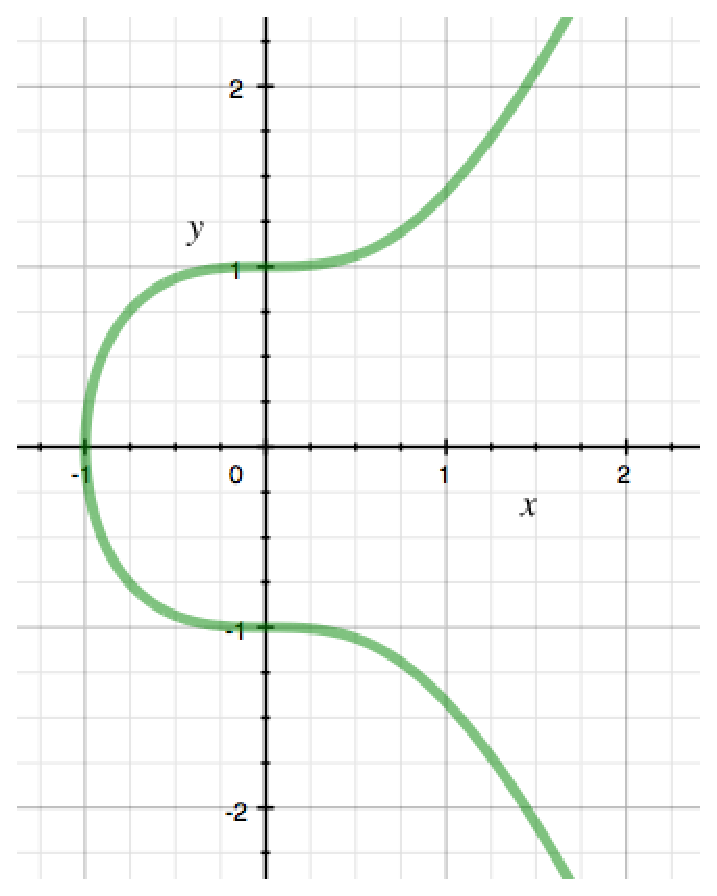
\includegraphics[width=0.2\textwidth]{ex1.eps}
\end{center}
\vspace{-0.2in}
\caption{A manifold with intrinsic dimension $1$ and extrinsic dimension $2$.}
\label{fig:1}
\end{figure}
\vspace{-0.2in}
\begin{figure}[h]
\begin{center}
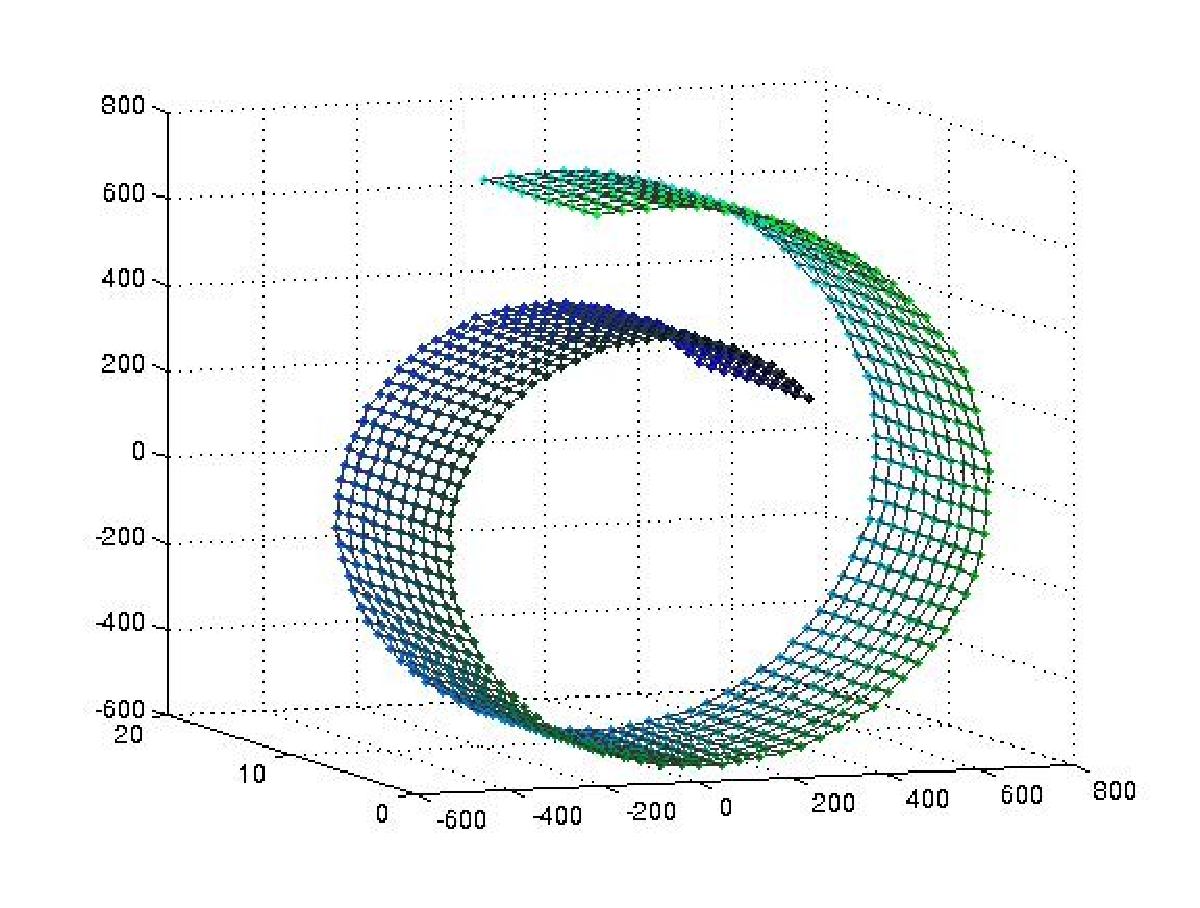
\includegraphics[width=0.3\textwidth]{ex2.eps}
\end{center}
\vspace{-0.2in}
\caption{A manifold with intrinsic dimension $2$ and extrinsic dimension $3$.}
\label{fig:2}
\end{figure}

Intrinsic dimension refers to the dimension of the manifold itself, and does
not depend on the space in which the manifold lives. If we have an ant walking
along the curve in Figure 1, we can identify a point by the
time at which the ant reaches that point. Thus, the manifold has intrinsic
dimension $1$. We can identify a point on the `Swiss roll' manifold in Figure 2
by drawing a grid on the surface and specifying the two grid lines that
intersect at that point. Thus, the manifold has intrinsic dimension $2$.

Thus, mathematicians tend to refer to $k$-manifolds in $\R^n$ ($n$-dimensional
space). The shape of a manifold is formally captured by finding a one-to-one
correspondence or transformation (called a {\bf homeomorphism}) between the
points in the manifold and $\R^k$. The intuition is that, if one zooms in
close enough to any point of a $k$-manifold, it should approxmiately resemble a
small portion of $\R^k$, perhaps bent, but not cut or glued. This means that a
figure eight is not a manifold, because, no matter how far you zoom into the
center, you see not a line (like $\R^1$), but rather two lines crossing. Figure
3 visualizes a homeomorphism between part of $\R^2$ and part of a $2$-manifold
in $\R^3$.
\vspace{-0.2in}
\begin{figure}[h]
\begin{center}
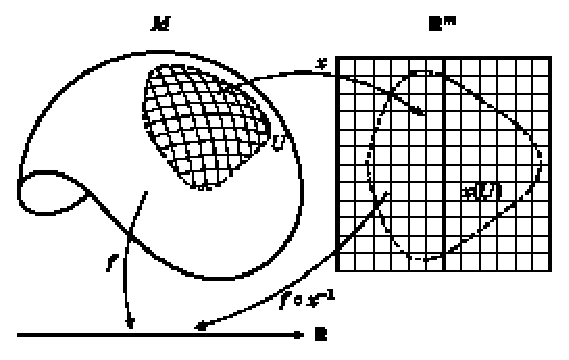
\includegraphics[width=0.3\textwidth]{homeomorphism.eps}
\end{center}
\vspace{-0.2in}
\caption{A homeomorphism}
\label{fig:3}
\end{figure}
\vspace{-0.1in}

\noindent
Audience 2 - Somya Singh, my 13-year old sister

Mathematicians use the word {\bf manifold} to refer to certain kinds of smooth
shapes. Most of the shapes you can think of are manifolds: pentagons, circles,
lines, boxes, spheres, etc.

Manifolds have a property called dimension.
One way to think about dimensions is to build them from the ground up, as in
the picture below. A point is zero dimensional; it's the basic building block.
If we take a two points and connect them, we get a line segment, which is
$1$-dimensional. If we take two identical line segments, connect the endpoints,
and fill in the space, we get a rectangle, which is $2$-dimensional. If we take
two identical rectangles, connect the corners, and fill in the space, we get a
box, which is $3$-dimensional. By repeating this process, we can
get even higher dimensional shapes, which you can't picture too well.
\vspace{-0.1in}

\begin{figure}[h]
\begin{center}
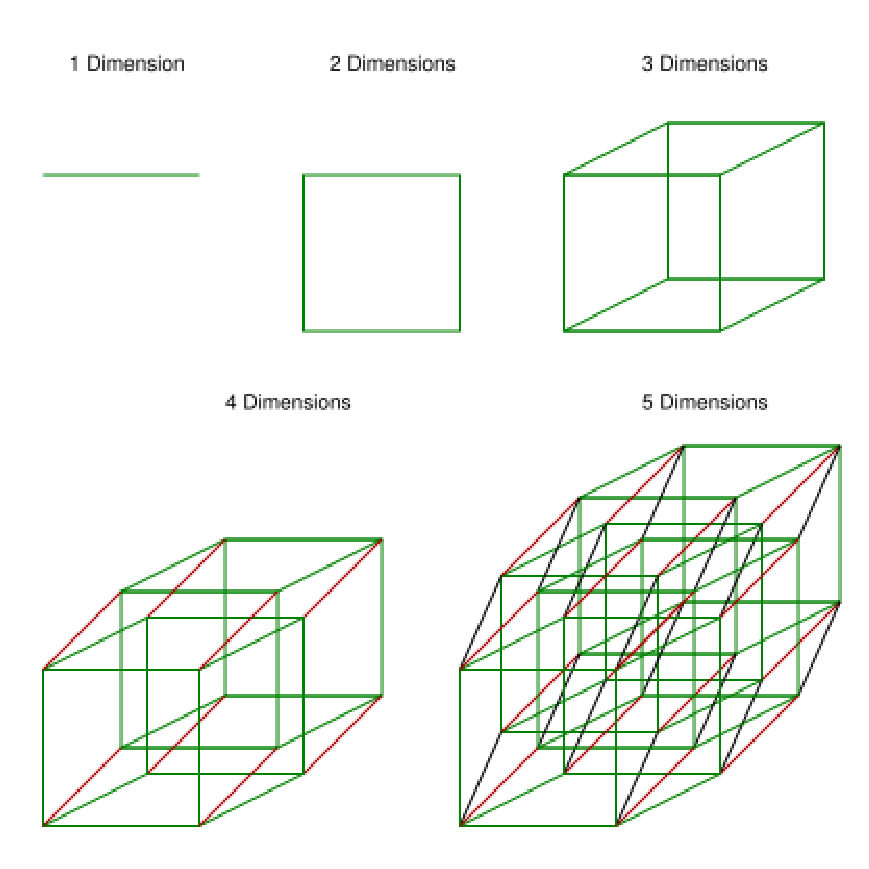
\includegraphics[width=0.34\textwidth]{dimension.eps}
\end{center}
\vspace{-0.2in}
\caption{Dimensions}
\label{fig:4}
\end{figure}
\vspace{-0.2in}

The dimension of a manifold is the dimension of the shape you have to
bend to make that manifold. If you draw a circle but don't color it in, you
have a $1$-dimensional manifold in $\R^2$, because the circle is like a bent
line in a plane. If you color the circle in, you get a $2$-dimensional
manifold in $\R^2$, because you can bend the edges of a rectangle to make a
circle.
\end{document}
